
\documentclass[a4paper, 10pt]{article}
\usepackage[utf8]{inputenc}
\usepackage{minted}
\usepackage{xcolor}
\usepackage{graphicx}
\usepackage{indentfirst}
\usepackage{epigraph}
\usepackage{url}
\usepackage[colorlinks=true, linkcolor=blue, urlcolor=blue]{hyperref}

\title{The Lure of Emerging Virtual Computers}

\author{Reza Hasanzadeh\thanks{This work has been funded by a generous grant from the \href{https://my.ethswarm.org/grants}{Swarm Assosiation}.}  \\ \href{mailto:rezahsnz@proton.me}{\small{rezahsnz@proton.me}}}

\date{\footnotesize{Draft} \\ \footnotesize{November, 2022}}

\begin{document}

\definecolor{fairgreen}{rgb}{0, 0.3, 0.15}

\maketitle

\epigraph{For an hour, Evans took the system through its paces, showing the writer
how it was possible to manipulate text, retrieve information, and
collaborate with others. At the end of the demonstration Kesey sighed and
said, "Its the next thing after acid."}{\textit{What the Dormouse Said} \\ \textit{How the Sixties Counterculture Shaped the Personal Computer Industry} \\ \textit{JOHN MARKOFF}}

\section{Preamble}
Computing has always been a battleground for two opposing ideas: \textit{batch processing/time-sharing} vs \textit{interactive/personal computing}. Batch processing reigned from the dawn of computing up until mid 70s. With mamoth expensive computers occupying several stories of a building, the idea of owning a whole computer was not a possibility for individuals. During this period, the only option for people to use computers, whose availability was often one per university, was to sign up in advance for some computer time. As technology advanced, however, and due to an interesting effect called Moore's law, computing started to become democritized. Ultimately during mid 70s, personal computing took momentum and became the new king infesting every home, every desk, and even every pocket. During all these years since the dawn of computing, people have always tried to simulate batch processing on pesonal computers or vice versa. The battle got more interesting with the adoption of the Internet. Now people could link and form larger groups of interest offering more than what was possible on any single personal computer. Napster, BitTorrent, SETI@home, Gnutella, Bitcoin, and ... are few examples of the temptation to simulate resource-sharing on personal computing later became known as peer-to-peer computing. \cite{milo:2002} surveys some of these systems. Today, peer-to-peer computing is omni-present and people, are craving again for good old days of powerful computers of the future. Building on the resiliency and availability of peer-to-peer systems, abstractions can be conceived that allow for new models of computers to be tried. This note is themed with such cravings and calls for a revolt against the state of today's computing.

\section{Building blocks}
Incentivized peer-to-peer systems started to pop up once Bitcoin and more advanced networks like Ethereum proved viable. Ethereum advances Bitcoin's storage system and allows more fine grained control over the storage of integers through systems of smart contracts. This permission-less self-regulation of assets is promising in that more complex objects could also be managed consensually. Ethereum virtual machine is a turing-complete computer capable of simulating almost any phenomenon in the world. This power, however, cannot be exercised in every domain. Take the simulation of an earthquake for example, it would take a lot of resources for this model to be represented and evolved within the Ethereum blockchain. The solution to this problem, if it is needed to be solved through decentralised technologies, is to divide it into parts and get them treated separately by special purpose networks. Storage and computation are the building blocks of any activity with the storage itself being the timely facet of computation, a communication from past to the future\cite{Lampson:2006}. So, in reality every activity is a form of computation. An object's lifecycle includes creattion, manipulated, storage, and finally disposal. So it seems logical to concieve of computation and storage facilities on top of blockchain technology. Swarm\footnote{\url{https://www.ethswarm.org}} and Golem network\footnote{\url{https://www.golem.network}} are two promising initiatives that aim to bring permission-less and privacy respecting storage and compute functionalities to users.
\par
\textbf{Swarm} --- Swarm\cite{swarm:2021} is network of peer-to-peer computers(nodes) joined together to form a unified  information storage and communication facility. Storage involves dividing data into small chunks(usually 4KB in size) and distributing them over the whole network in a way that storage is reliable and retrieval is quick. Each chunk ends up being stored on different node(s) to ensure resiliency against single node failures. Each file is addressed using the hash value resulting from its \texttt{Balanced Merkle Tree} representation. This storage and addressing shceme is commonly known as \texttt{content addressing} which in essence eliminates the need for extra metadata about the location of the stored data with the added benefit of robust integrity checks. To store data, one needs to buy the rights to write into the storage space which is known as postage stamps. The medium of exchange within the Swarm network is called the BZZ token\footnote{BZZ is an ERC-20 token and the medium of exchange within the Swarm network.} that acts as the incentive paid to the storage providers in return for their physical contributions to the netwok. This properly-incentivized, resilient, and privacy-respecting setup paves the way for more abrstract interfaces to appear on top of it.
\par
\textbf{FairOS-DFS} --- Swarm's interface, though sophisticated, is still clumsy for humane uses. This is where FairOS-DFS comes to rescue by introducing advanced interfaces that allow a rich basket of applications to be created in a shorter amount of spacetime. Figure  \ref{swarmfair} demonstrates the relationship between Swarm and FairOS-DFS and the set of interfaces available for application developers\footnote{\url{https://docs.fairos.fairdatasociety.org/docs/fairOS-dfs/introduction}}. As is seen on the figure almost all the storage related functionalities are baked into the DFS layer. Out of all of them, the function of the \texttt{pod} seems to be of major importance. Pods play a central rule within the DFS layer where most write/read operations need them to exist and be accessible. Pods can also be thought as logical drives; a directory structure similar to a filesytem enabling file objects to be stored on Swarm. If an application is a directory structure composed of many files and directories, for example, then each application can be stored on Swarm as an standalone pod. Pods can communicate with one another through sharing parts(e.g. a file within the pod) or all of the pod with the outside world. The identification of pods are done through their \texttt{names} with no two pods sharing the same name within a user's wallet. Pods are private to users unless they decide to make them available to the outside world. This is done through a sharing mechanism. Once a pod(or a file within it) is shared, a \texttt{reference key} is generated that allows others to get a copy of the pod. Though simple, the notion of the pod enables a rich league of interacting objects to be sowed on the fertile soil of Swarm lands where the emergence of a \textit{brave new world} of virtual computers is inevitable.
\begin{figure}
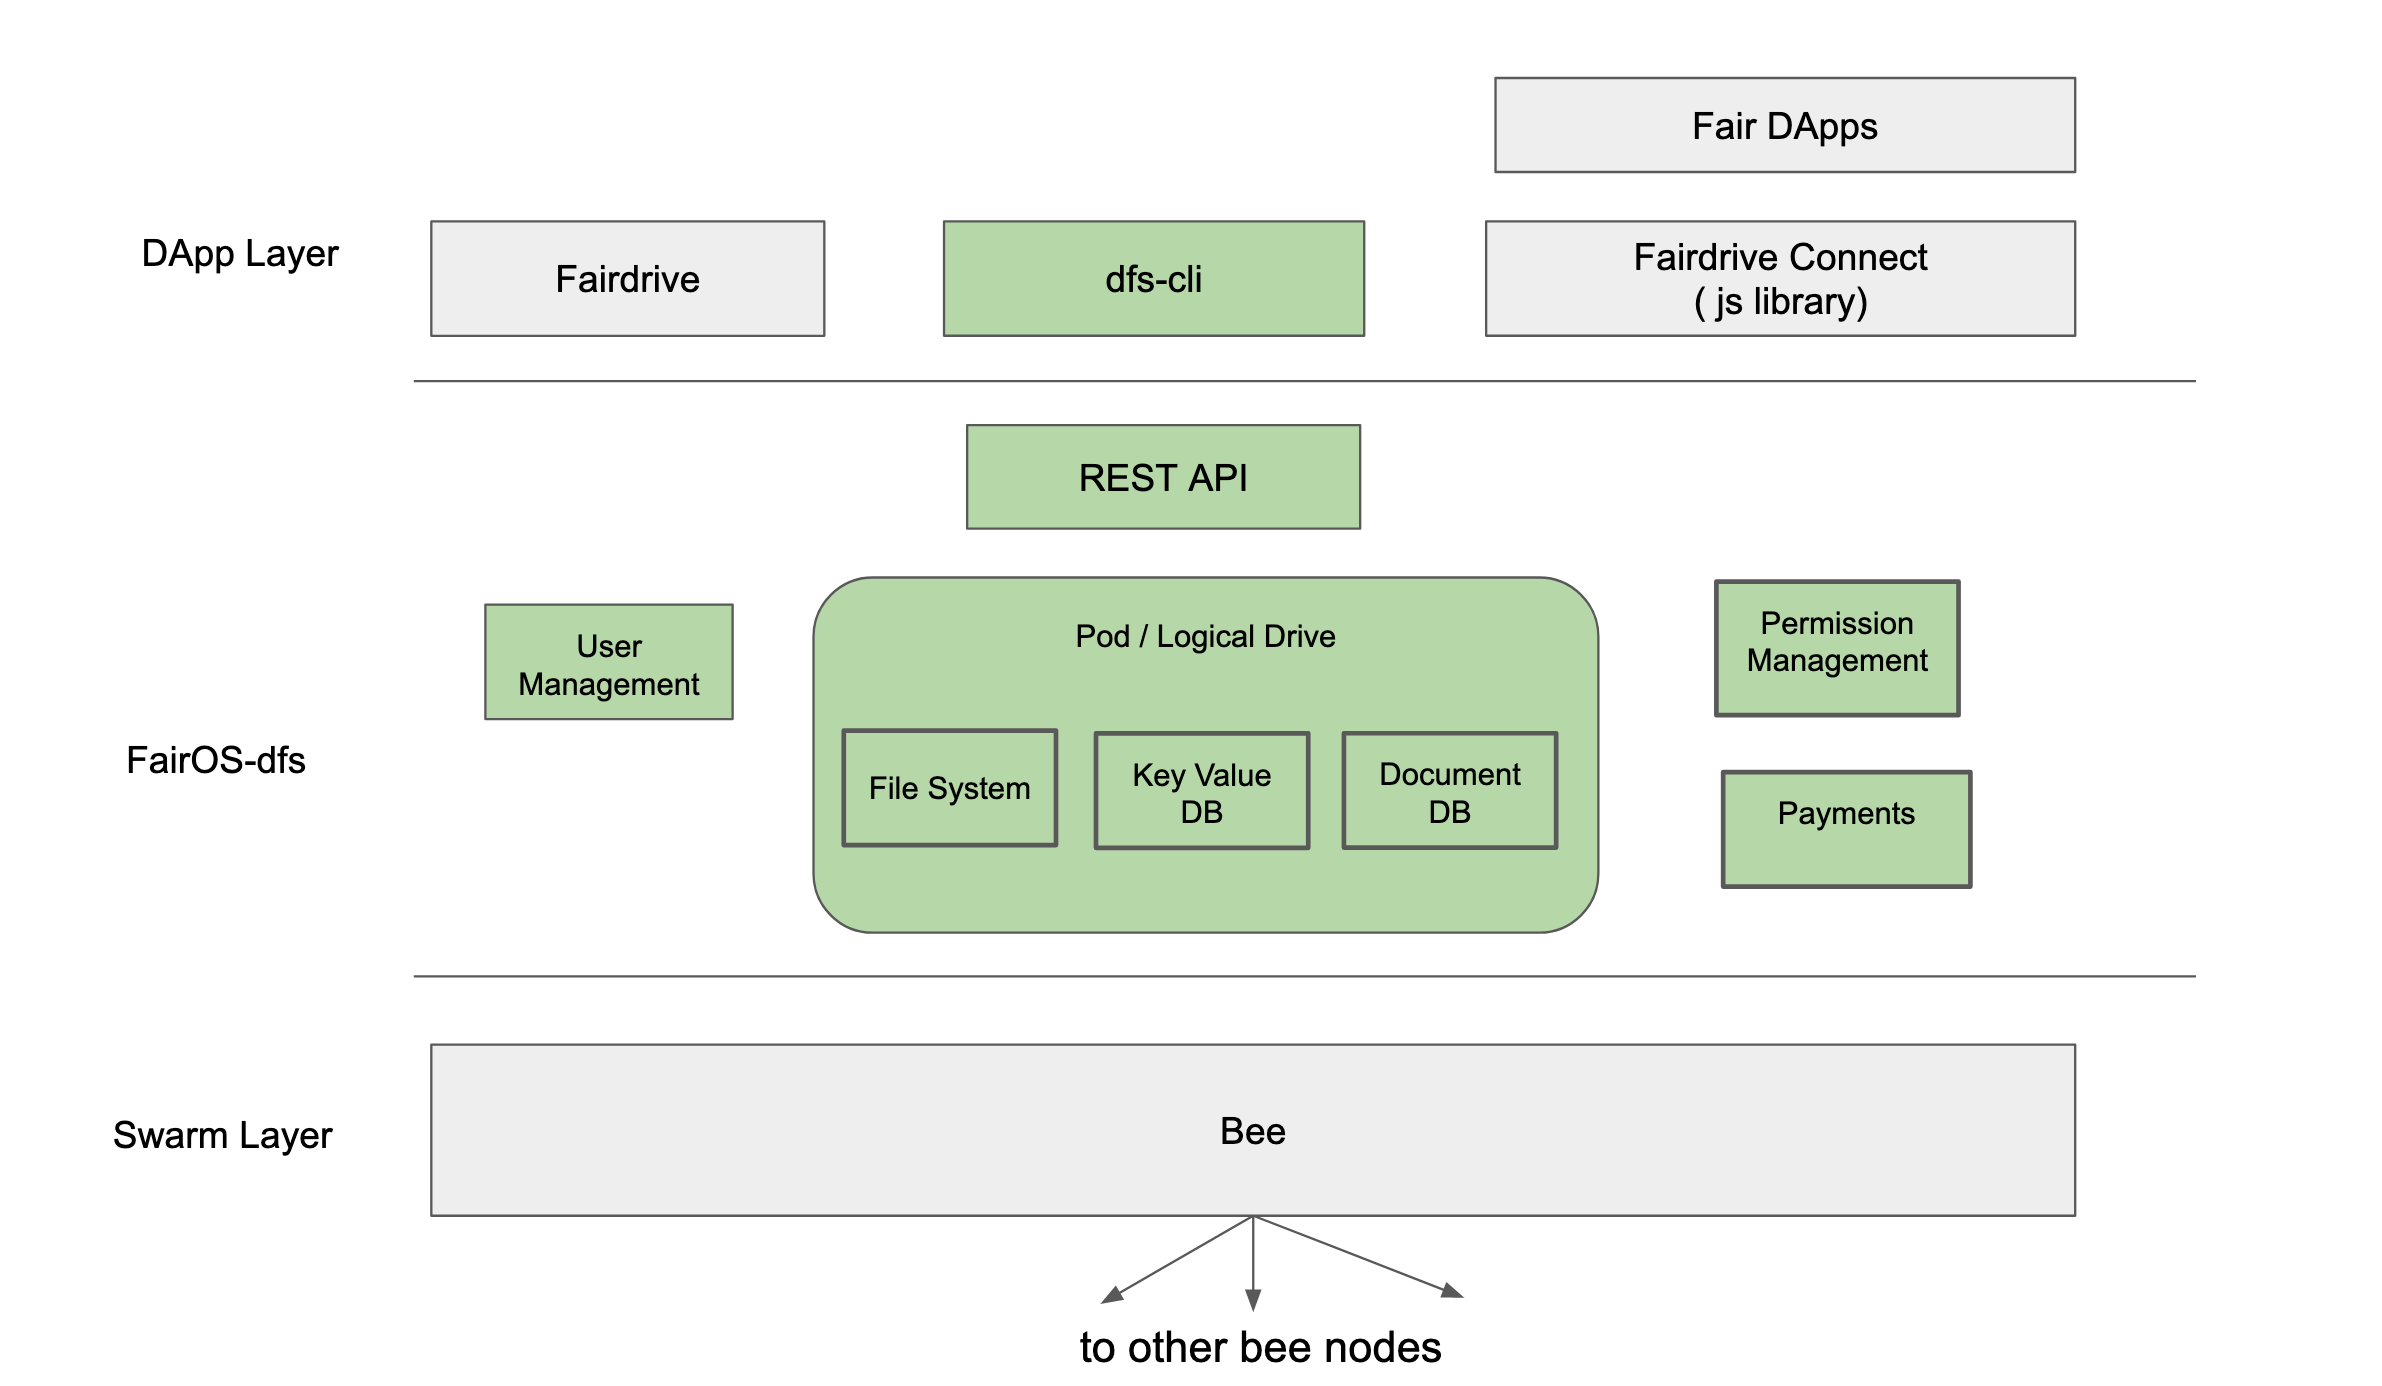
\includegraphics[scale=0.3,keepaspectratio=true]{images/swarm-fair.png}
\caption{\label{swarmfair}Swarm and \textcolor{fairgreen}{FairOS-DFS}}
\end{figure}
\par
\textbf{Golem} --- Golem network is a peer-to-peer marketplace for \textit{batch} compute jobs. It consists of three entities: requestors who need and pay for compute resources(cpu, ram , ...), providers who offer their compute resources in exchange for money, and a matching agent called the \texttt{YAGNA daemon} that mediates between requestors and providers. A compute job is initiated by a requestor who makes a demand specifying the minimum amount of resources(e.g. 24GB of ram) needed along with the budget in GLM\footnote{GLM is an ERC-20 token and the medium of exchange within the Golem network.} and waits for any provider to accept her criteria. Once an aggrement is reached, the provider loads the execution environment(a golemized-docker image already prepared and registered within the Golem network) and starts running the job. When the execution of the job is finished, the requestor collects the output (and any logs) and pays for the services she has used. The following three sections briefly describe the important participants of the Golem network.
\par
\textbf{Requestor} is an umbrella term for a set of agents working together to make a compute job happen. Golem network operates on the Ethereum network with support for other EVM-compatible blockchain like the Polygon network. The first step for a requestor is to have a valid wallet loaded with enough funds to sign transactions and pay the compute bills. Then comes the need to prepare an execution environment within which the logic of the compute job is going to be carried out. This environment is a Docker image that will be started by providers once an agreement is reached. This image first needs to be golemized and added to the Golem's image registry. Then comes the actual logic of a compute job: a set of Python\footnote{Support for Javascript code is also provided} files, data files, and shell scripts that manage the compute job. File exchange channels brought up by YAGNA allows a requestor to send any files to the execution environment. These exchanges can happen from the start of the job all through the end of it, first sending data and code and then collecting outputs and logs. Once the compute job is finished, the bill is ready to be paid.
\par
A \textbf{provider} is simply a fraction of a computer's resources that is ready to be used within the marketplace set up by the Golem network. Just like the requestors, providers use the channels relayed by the YAGNA daemon for communicating with other network participants. A provider needs a wallet, some virtualized-ready operating system services, and a fraction of the resources to serve requestors. Providers often publish their offers in response to demands advertised on the network and when the agreement is reached, they start doing the job and get paid for it. Recall that the medium of exchange in Golem network is GLM and the rates are denominated in GLM/hour. Providers can change rates anytime and this flexibility is a double-edged feature: set rates too high and no one would be interested in your services, set them too low and you risk being unable to pay electricity bills. This is exacerbated by the volatile nature of the GLM token as the price of GLM is subject to market conditions. So, providers should  keep an eye on the price of GLM and adjust the hourly rates to make sure their offers are reasonable.
\par
Golem network is a peer-to-peer marketplace for compute jobs. A demand for a compute job is first published on the network and then offers are collected from providers. A typical offer includes a proposal that contains the specs of the hardware along with the rates for services. Of all offers received, the least expensive one is usually chosen and agreed with though this strategy can be changed customized by requestors. Once an agreement is reached, the budget for this job is locked by the YAGNA and when the job is finished, gets transferred to the provider. The YAGNA daemon mediates these communications between providers and requestors. The requestor's side of the mediation is composed of the YAGNA HTTP server along with client toolkits in the form of Python and Javascript libraries for communicationg with the HTTP server. The provider's side of mediation too consists of a daemon that waits for incoming demands, makes proposals to requestors, and manages all wallet related tasks.

\section{Reassemble}
Swarm and Golem are independent networks each covering a specific need. They can also be viewed as isolated parts of a giant computer. This view could be translated into solutions that try to combine the benefits independent decentralised tools offer. The following sections introduce such solutions. Later on, a framework is presented that bids for a new model of computers whose emergence we feel like to be inevitable in the coming years. The framework ideates computers as non-divisible units of measurement within a rich message passing network.
\par
\textbf{Compute pods} --- The notion of compute pods is an attempt to connect the worlds of peer-to-peer compute and storage networks: with FairOS-DFS acting as the storage wing and Golem as the computation wing. A compute pod simply contains a Golem application and directions on how to activate it on an actual Linux subsystem. Activation is done by invoking the Sovr CLI\footnote{\url{https://github.com/rezahsnz/sovr}} and issuing commands that operate on a JSON file called the \texttt{recipe}. The following snippet shows a typical recipe of a Golem application for recognizing images:
\begin{minted}[breaklines, fontsize=\footnotesize]{js}
{
  "name": "XCeption",
  "description": "A XCeption model for image classification based on Keras applications",
  "version": "1.0",
  "author": "tony76",
  "public": true,
  "golem": {
    "exec": "python3 [@]script/script.py --model xception --images [@]payload/external/images",
    "payload": [
      {
        "ref": "da41f8dfd57e2e89df2dacd3b01c4a1dbc7c4a1df429f96743317e6a220c5fac",
        "data": "/images.zip"
      }
    ],
    "output": "output",
    "log": "logs"
  }
}
\end{minted}
\textcolor{teal}{golem} property defines how the golem application gets the payload(input), runs, and finally produces the output and logs. The output and the logs of the compute pod are put in the directories pointed to by \textcolor{blue}{output} and \textcolor{blue}{log} properties with the possibility of sharing the output once it is ready. \textcolor{blue}{exec} contains the actual running command used to run the compute pod on Golem. \textcolor{blue}{payload} property can either be a local directory or a public pod. \textcolor{blue}{description}, \textcolor{blue}{version}, and \textcolor{blue}{author} properties serve as metadata here and can be omitted without causing any problems. \textcolor{blue}{name} property acts as the identifier for the pod within a user's DFS space. And finally, \textcolor{blue}{public} property, if set to \textcolor{brown}{true}, shares the compute pod with the outside world when it gets persisted.
\par
A tool called \texttt{Sovr CLI} is used to interpret the recipe file and provides three basic services: \texttt{persist}, \texttt{fork}, and \texttt{run}. Persisting saves a copy of the compute pod, which at the moment is a directory structre in local storage(e.g. \textcolor{darkgray}{/home/tony67/cpods/ml/xception}), to DFS and shares it if requested. Forking involves bringing a shared compute pod to the user's DFS first and downloading the pod to the local storage then. Running sends the compute pod to Golem to be run as a job. Note that before the compute pod is sent to Golem, all external payloads need to be resolved(forked and copied to local storage).
\par
\textbf{External payloads and tasks} --- Compute pods are bound to DFS and communicate in three ways: by \textit{being shared}, \textit{requesting external payloads}, and \textit{sharing their output}. To share a compute pod is synonymous with a weak broadcast message to all DFS users that something worthy of attention is born. The weakness stems from the fact that once something is shared on DFS, the dissemination of the reference key is upon the initiator. Having the reference key of a compute pod, anyone can get a copy of it and tailor it to her needs. Sharing the output is similiar to sharing an entire compute pod, the reference key needs to reach out to others in order for the output to be used. External payloads are public pods that are treated as dependencies and provide additional input for compute pods. They need to be brought in before a compute pod can feed on them which is the task of Sovr CLI. This mixture of local and external payloads allows to create complex workflows where big problems are divided into small ones and solved by separate compute pods. Sovr CLI refers to this as chaining compute pods and call it a task (figure  \ref{task}). A \texttt{task} is a sequence of compute pods where the output of a compute pod is fed as payload to the next compute pod in the sequence. A task description file is a simple JSON file that defines a task and instructs the order in which compute pods have to run. Having a set of compute pods and a plan to use them enables for far more complex workflows to be thought of beyond the reach of any single compute pod. Each stage of the workflow can be assigned to a compute pod and the order in which compute pods are run can be decided according to an arbitrary plan like a sequential order. Note however that the sequential ordering of compute pods within a task mentioned here is just one of many conceiveable plans for a task's composition.
\begin{figure}
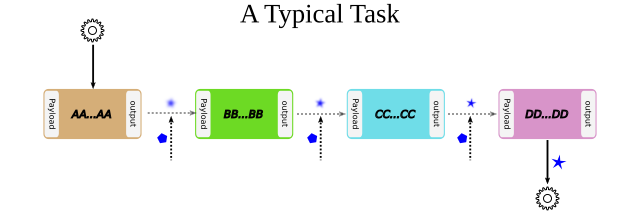
\includegraphics[scale=0.7,keepaspectratio=true]{images/task.png}
\caption{\label{task}Composition of a task}
\end{figure}
\par
\textbf{Communications enriched} --- Decentralised storage networks triumph dormant communications. A message is left somewhere deep within the realm of content addressed cyberspace waiting to be picked up before it gets garbage collected. While beneficial for certain use cases, this dormancy curbs the agility needed for OOP(object oriented programming)\cite{kay:1996} where messages are expected to be exchanged with the speed of light. Message passing is the central theme of  a salted OOP we adopt here where each object is a nondivisible virtual computer armed with sophisticated communication apparatus. A virtual computer is a dynamic volume of logics capable of changing its shape when exposed to certain messages(deviating away from the accepted notion of textual descriptions). It can grow in response to embedding a message, shrink upon receipt of a message annoucing deprecation of some parts, or re-organize itself upon receipt of newer versions of body parts. By message here, we mean any form of communications: from a simple request of evaluating "(cons '4 '(9 16 25 36 49))", to a new version of an experimental hippocampus just released to boost memory retention of cybercats. A virtual computer could be an interpreter for a LISP dialect or a stray cat roaming the medium looking for mates. The medium itself is a giant simulation machinery formed by a network of physical computers that relay messages for fun and profit and is capable of realizing strange worlds.
\par
\textbf{Messages} --- A message is a dynamic notice composed of: contents, instructions for decoding the contents - a decoder, and metadata about the message. There are no upper bounds on the size of a message. A message can be as simple as containing a single decimal number or as complex as a detailed simulation. A message, if complex, is expected to provide necessary tools right within itself for its content to be decoded properly. Consider a robotic limb, for example, that has just been released and is ready for adoption. The key step for adoption here is to let potential users try the package before any decisions. The decoder for the robotic limb could be a bare-bone robot package that facilitates various tests to be conducted on the limb; sort of a sandboxed simulation environment for limb tests. Later if test results turned out satisfactory, any fleet of robots can get the new robotic arm and upgrade themeselves. Messages can take the form of standalone virtual computers too. This means that we can actually send virtual computer around, polishing off boundaries between messages and virtual computers. We like to call it \textit{weak messaging} when messages are plain pile of bytes and \textit{strong messaging} when messages are actual virtual computers. Consider the case of emulating a retro gaming console: one message can emulate processor, another memory, another I/O, and finally messages are needed that house cartridge of games. A message occupies some space within the medium, so the whole process of acceptance and rejection of messages should conform to some N-dimensional pattern matching rules. This scheme promises a self-regulating medium where virtual computers can dynamically reshape themselves in response to foreign stimulae, all thanks to rich messages flying around. If any such scheme is adopted, the end product would be teeming compute lego sets that self-regulate via exchanging messages. 
\par
\textbf{Virtual computers} --- Messages carry dynamics of change and deliver them to virtual computers. A virtual computer is a recursive mass of dynamism that hosts several virtual computers and provides them with an environment to communicate towards achieving a common goal. Unlike their real world counterparts, virtual computers are very flexible and can change their shape and therfore their function far more quicker. A virtual computer gets reshaped once a new message is internalized or an old part is deemed obsolete and is stripped. Symmetrical to internalizing, stripping involves wrapping the unwanted part as a message and broadcasting it through the medium. The stripped message is either internalized somewhere else or removed from the medium. This dynamic reshaping translates to a N-dimensional mathematical representation addressable within and bounded by the medium. This mathematical representation has the benefit of standardizing discovery of messages. Special objects(or virtual computers) are employed and briefed by virtual computers with the task of constantly searching the medium for potential new listings of messages. These objects have the ability of selecting potential messages by testing them against metrics they have already been briefed about. This is however only possible for those messages which contain proper decoders. If a message has no decoders, there is no way for it to be tested and thus internalization gets hindered. Compared to internalizing, stripping needs no special agents and so is very energy efficient: an object gets removed from the virtual computer and is no longer cared for. 
\par
\textbf{The medium} --- Communications, even crude forms, is at the heart of computing. The term \textit{medium} discussed so far refers to any group of virtual computers that know how to find one another and exchange messages. At first the medium is an empty network consisting of just special objects called \textit{genesis objects}: bare-bone virtual computers having a messaging interface which implements specifications of the communications protocol. Genesis objects are easy to get. If the medium is content addressed, their locations can be inferred from digests of protocol specification files. On the other hand, if the medium is not content addessed or location inferral is not possible, well-known locations can be chosen for them and made available publicly. Once a genesis object is obtained, it gets internalized(or forked to be exact) within the mother virtual computer and assumes the role of messaging interface henceforth. The medium is a live entity and evolves every moment. Few moment into the life of the medium, it is expected to observe that some virtual computers will begin to form niche groups calling for interested ones to join them. The medium provides groups with resources to set themselves up and advertise. Each group should then make a banner describing the objectives of the group and steps required to subscribe to its events. When the medium is mature, we also expect to see interesting groups that are doing utility and maintenance jobs like stripped virtual computers scavengers, volunteer test takers for newly released objects, and etc. The boundary between the messages and virtual computers within the medium is truly thin. A simple message, for example "Hello, World!", is not a pile of bytes flying around, but an actual virtual computer that when activated, constantly outputs "Hello, World!". So, the medium is only dealing with virtual computers and they are the \texttt{smallest unit of computation} in existence. The medium would not embrace swapping the rich notion of virtual computers for some blunt pile of bytes just because storing and exchanging them would be more spacetime friendly. Virtual computers here, are dynamic objects pregnant with vibrant processes. 
\par
\textbf{An approximation} --- Realization of a medium for virtual computers discussed above may be a bit out of reach at the moment. Given that we do not yet have mathematical constructs vigorous enough to represent virtual computers, we have to set sails and at least try to approximate the medium with what we have at our disposal: \textit{compute pods}. Swarm and FairOS-DFS form the base layer for storage and Golem provides the base layer for batch compute processing. To start, compute pods can assume the role of virtual computers. Indexing bots are needed to constantly look for public pods and brief others about. To enable groups and subscription to events, several publicly announced wallets are needed that hold (compute pods) those groups. This is a bad design of course, after all everybody can write into and mess things up. Certain measures can be taken though that raise the cost of writing into those pods: centralization of groups' control could be one of them. Certain bots are needed to carry messages around. Message exchange should not be free because spamming has to be rendered expensive. And finally, a marketplace can be created where users freely buy and sell compute pods.

\section*{Conclusion}
Compute pods are an attempt to fuse the worlds of decentralised storage and compute. They enable us to store dormant computers on decentrlised storage facilities provided by the Swarm network. Once awaken on an actual computer, a compute pod gets run on the Golem network. Compute pods can be shared and forked, enabling collaborative software development. This is not the end though and an army of compute pods can be grouped together in what we call tasks to solve complex workflows.
\par
This note was the first in the series of essays whose objective is to come up with a new kind of computers. Virtual computers are flexible objects that form a network where message exchange is the primary theme of communication. Messages, however, are rich, meaning that they are actual virtual computers passed around. Virtual computers absorb in-bound messages, shed obsolete parts as out-bound messages and therefore reshape when exposed to messages. The shape of a virtual computer is best represented by some N-dimensional mathematical construct addressable within the fabric of the medium. The whole promise of virtual computers is to treat computers they way they are: forget about data structures and instead focus on actual computers as minimum units of measurment. This could be one step forward towards the goal of exploring new horizons conventional computing has yet to fantasize about. The real challenge virtual computers face is to figure out how to encode themselves in a way that is mathematically rigirous. Topological constructs seem as potential candidates for consideration as they harbour many levels of dymanism and are simple to describe too.

\bibliographystyle{apalike}
\bibliography{refs}

\end{document}
